\chapter{ผลการทดลอง}
\label{chapter:result}

ผลลัพธ์การทดสอบประสิทธิภาพในวิธีการใหม่ของเราและเปรียบเทียบกับงานวิจัยอื่น ๆ ที่เกี่ยวข้อง แสดงในตารางที่~\ref{Table:ExperimentalResults} จากตารางดังกล่าว วิธีการของเราได้รับ F-measure สูงที่สุด ที่ 0.506 ซึ่งแสดงให้เห็นชัดเจนว่าวิธีการของเรามีประสิทธิภาพดีกว่าวิธีการ SWT ต้นฉบับ~\cite{5540041} ยิ่งไปกว่านั้นวิธีการของเรายังได้รับ F-meaure ที่มากกว่าวิธีการ BG+ImN~\cite{7532890} และ BG+I2V~\cite{7532890} ซึ่งทั้งสองวิธีนี้ใช้เทคนิค Deep Learning เป็นส่วนหนึ่งในการตรวจหาข้อความในภาพ อย่างไรก็ดีค่า Precision และ Recall สูงสุดของการทดลองนี้อยู่ที่ 0.715 และ 0.481 เป็นของ BG+I2V และ BG+ImN ตามลำดับ สำหรับตัวอย่างพื้นที่ของข้อความที่วิธีการใหม่ของเราตรวจพบถูกแสดงในภาพ~\ref{Fig:ExampleResult}

\begin{table}[!h]    
    \centering
    \begin{tabular}{lccc}
        \hline
        Method & Precision & Recall & F-measure \\ \hline \hline
        STD~\cite{6628665} & 0.165 & 0.051 & 0.078 \\
        SBD~\cite{6761596} & 0.180 & 0.102 & 0.130 \\
        TLD~\cite{rigaud:hal-00841492} & 0.095 & 0.095 & 0.095 \\
        BG + ImN~\cite{7532890} & 0.451 & \textbf{0.481} & 0.466 \\
        BG + I2V~\cite{7532890} & \textbf{0.715} & 0.191 & 0.301 \\
        Baseline~\cite{5540041} & 0.068     & 0.336 & 0.113 \\
        วิธีการของเรา & 0.564     & 0.458 & \textbf{0.506} \\ \hline
    \end{tabular}
    \caption{ตารางแสดงการเปรียบเทียบประสิทธิภาพของวิธีการใหม่ของเราร่วมกับวิธีการอื่น ๆ ที่เกี่ยวข้อง}
    \label{Table:ExperimentalResults}
\end{table}


\begin{figure}[!h]
    \centering
    \subfigure[]{
        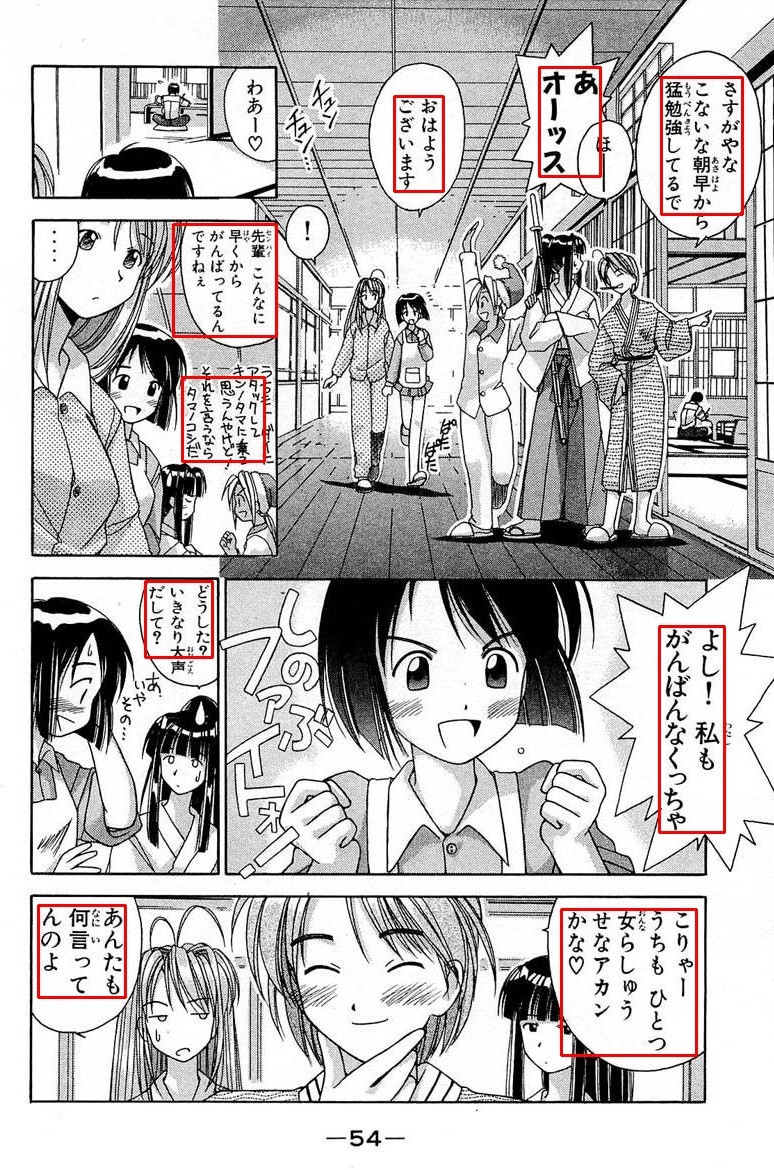
\includegraphics[width=0.45\textwidth]{images/result1.jpg}  
    }
    \subfigure[]{
        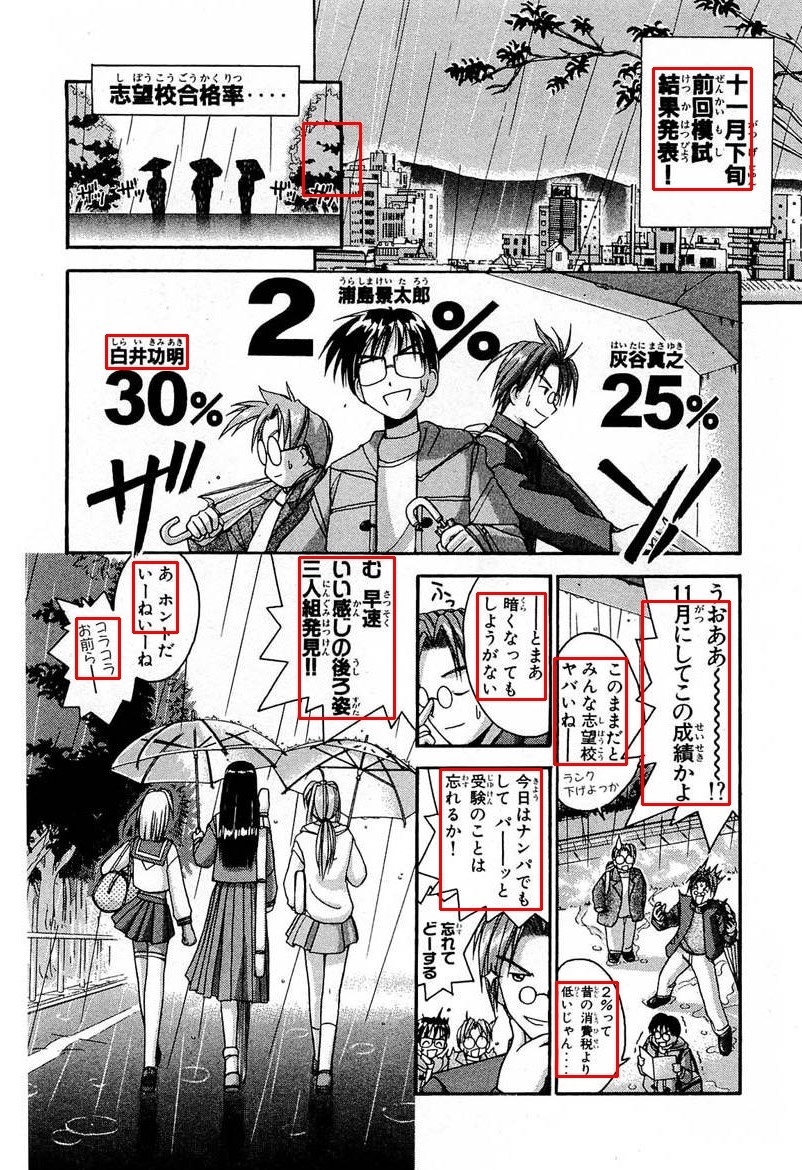
\includegraphics[width=0.45\textwidth]{images/result2.jpg}  
    }
    \subfigure[]{
        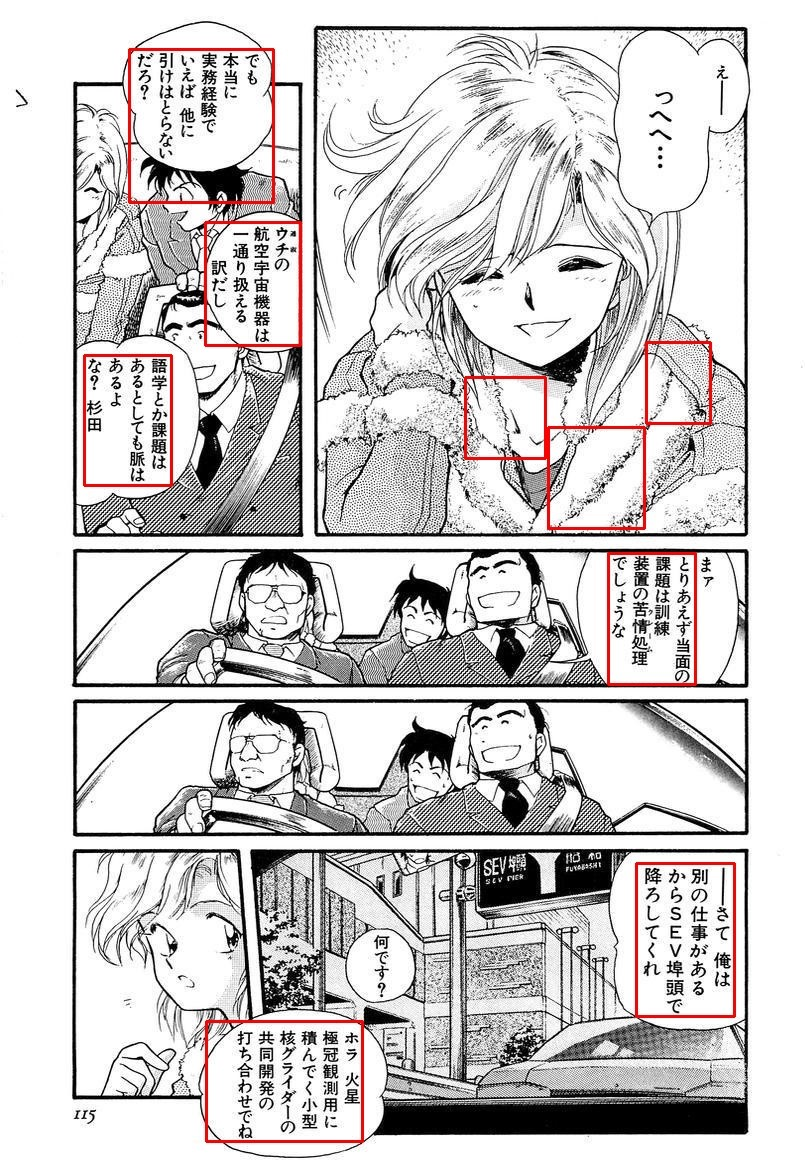
\includegraphics[width=0.45\textwidth]{images/result3.jpg}  
    }
    \subfigure[]{
        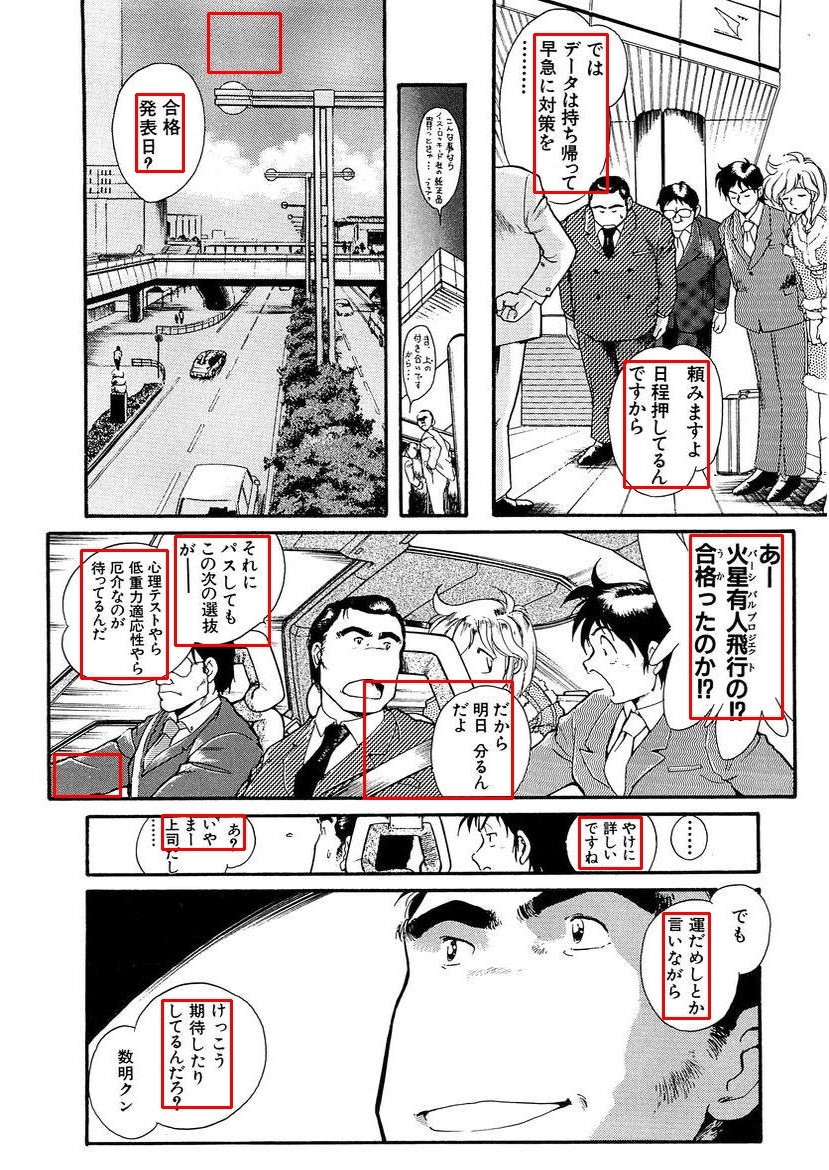
\includegraphics[width=0.45\textwidth]{images/result4.jpg}  
    }
    \caption{ตัวอย่างขอบเขตข้อความที่วิธีการของเราตรวจพบ (ก--ข) Love Hina \copyright Ken Akamatsu และ (ค--ง) Eva Lady \copyright Miyone Shi}
    \label{Fig:ExampleResult}
\end{figure}

เป็นที่น่าสนใจอย่างมากที่วิธีการของเราสามารถทำงานได้ดีกว่าเทคนิค Deep Learning ทั้งสองวิธี สมมติฐานแรกคือ BG+ImN นั้นใช้ ImageNet Classification Model~\cite{Krizhevsky} ซึ่งถูกเทรนบนภาพถ่ายของวัตถุจริง อย่างไรก็ดีภาพวาดมังงะของวัตถุต่าง ๆ นั้นมีความแตกต่างจากภาพวัตถุจริงอย่างชัดเจนซึ่ง ณ จุดนี้ทำให้วิธีการนี้ไม่สามารถทำงานได้เต็มประสิทธิภาพ อีกวิธีการที่ใช้ Deep Learning คือ BG+I2V ถึงแม้ว่าวิธีการนี้จะได้รับ Precision สูงที่สุดในการทดลองของเราแต่คะแนน Recal นั้นต่ำกว่าทั้ง BG+ImN และวิธีการของเรา วิธีการนี้ใช้โมเดล Illustration2Vec~\cite{Saito:2015:ISV:2820903.2820907} เป็นโมเดลสำหรับคัดแยกข้อความจากวัตถุอื่น ๆ ที่ปรากฎในภาพมังงะ ส่วนของโมเดลนั้นถูกเทรนบนภาพวาด Anime (ภาพการ์ตูนแบบญี่ปุ่น) และภาพมังงะจากหลากหลายแหล่งอันประกอบไปด้วย Danbooru และ Safebooru ซึ่งมีลักษณะงานคล้ายกับข้อมูลที่เราใช้ทดสอบในวิธีการของเรา แต่โมเดลนี้ถูกออกแบบมาเพื่อการทำนายป้ายกำกับ (Tag Prediction) และค้นหาภาพที่คล้ายคลึงกัน ดังนั้นการเลือกใช้วิธีการที่ไม่ต้องลักษณะงานโดยตรงในลักษณะนี้จึงอาจเป็นเหตุผลว่าทำไมโมเดลนี้จึงไมมีประสิทธิภาพเท่าที่ควรในการทดลองนี้
